%%%%%%%%%%%%%%%%%%%%%%%%%%%%%%%%%%%%

\section{正規分布}

%%%%%%%%%%%%%%%%%%%%%%%%%%%%%%%%%%%%

\begin{frame}
\frametitle{正規分布}

\begin{itemize}

\item 単峰で対称な、ベル型の曲線

\item 多くの変数はほぼ正規分布に従うが、完全に正規分布に従うものはない

\item \mathhl{N(\mu,\sigma)} と表す $\rightarrow$ 平均 $\mu$、標準偏差 $\sigma$ の正規分布

\end{itemize}

\begin{center}
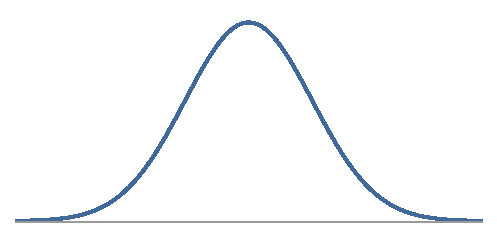
\includegraphics[width=0.7\textwidth]{4-1_normal_distribution/figures/simpleNormal/simpleNormal}
\end{center}

\end{frame}

%%%%%%%%%%%%%%%%%%%%%%%%%%%%%%%%%%%%

\begin{frame}
\frametitle{男性の身長}

\twocol{0.5}{0.5}{
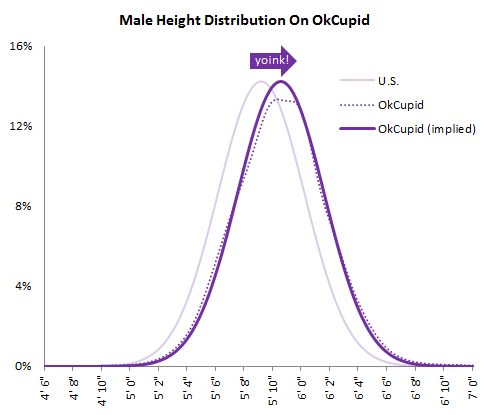
\includegraphics[width=\textwidth]{4-1_normal_distribution/figures/ok_cupid/ok_cupid_men} \\
}
{
{\footnotesize「OkCupid の男性の身長は、期待される正規分布にほぼ従っているが、全体的に右にずれている。男性はほぼ普遍的に数センチ多めに申告する傾向がある。」

「約5フィート8インチ付近から、点線の曲線の上部がさらに右に傾いていることがわかる。これは、6フィートに近づくにつれて男性が少し多めに切り上げていることを意味し、その羨望の心理的な基準値を目指している。」
}
}

\ct{\webURL{http://blog.okcupid.com/index.php/the-biggest-lies-in-online-dating/}}

\end{frame}

%%%%%%%%%%%%%%%%%%%%%%%%%%%%%%%%%%%%

\begin{frame}
\frametitle{女性の身長}

\twocol{0.5}{0.5}{
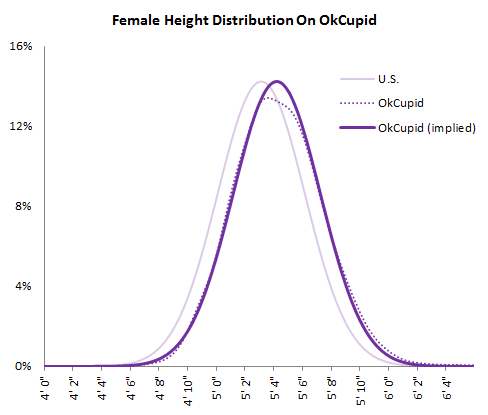
\includegraphics[width=\textwidth]{4-1_normal_distribution/figures/ok_cupid/ok_cupid_women} \\
}
{
{\footnotesize 「女性のデータを調べたところ、身長の誇張は同様に広まっていたが、特定の基準値に向けた急激な変化はなかった。」
}
}

\vfill

\ct{\webURL{http://blog.okcupid.com/index.php/the-biggest-lies-in-online-dating/}}

\end{frame}

%%%%%%%%%%%%%%%%%%%%%%%%%%%%%%%%%%%%

\subsection{正規分布モデル}

%%%%%%%%%%%%%%%%%%%%%%%%%%%%%%%%%%%%

\begin{frame}
\frametitle{パラメータの異なる正規分布}

\vspace{-0.5cm}
\begin{center}
$\mu$：平均、$\sigma$：標準偏差
\[N(\mu = 0, \sigma = 1) \hspace{1.4cm} N(\mu = 19, \sigma = 4) \]
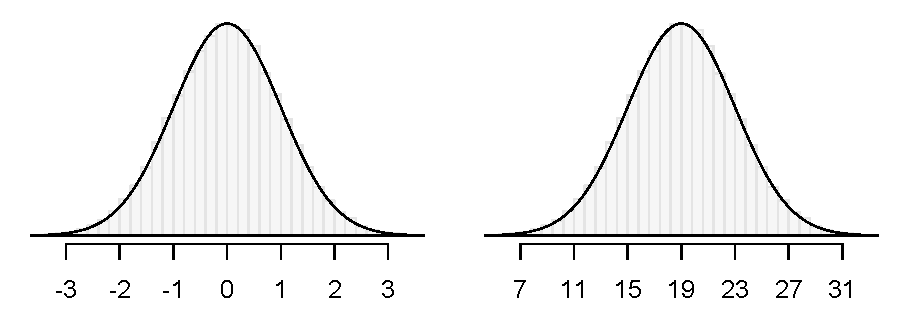
\includegraphics[width=0.6\textwidth]{4-1_normal_distribution/figures/twoSampleNormals/twoSampleNormals} \\
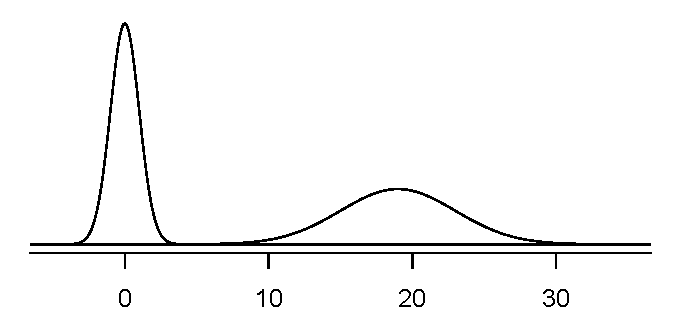
\includegraphics[width=0.6\textwidth]{4-1_normal_distribution/figures/twoSampleNormalsStacked/twoSampleNormalsStacked}
\end{center}

\end{frame}

%%%%%%%%%%%%%%%%%%%%%%%%%%%%%%%%%%%%

\subsection{Zスコアによる標準化}

%%%%%%%%%%%%%%%%%%%%%%%%%%%%%%%%%%%%

\begin{frame}
\frametitle{}

\dq{SAT のスコアは平均1500、標準偏差300の正規分布にほぼ従う。ACT のスコアは平均21、標準偏差5の正規分布にほぼ従う。大学の入学担当者が2人の志願者のうち、他の受験者に対してどちらが標準化テストでより良い成績を収めたかを判断したい。SAT で1800点を獲得したパムと、ACT で24点を取ったジムのどちらが優れているか？}

\begin{center}
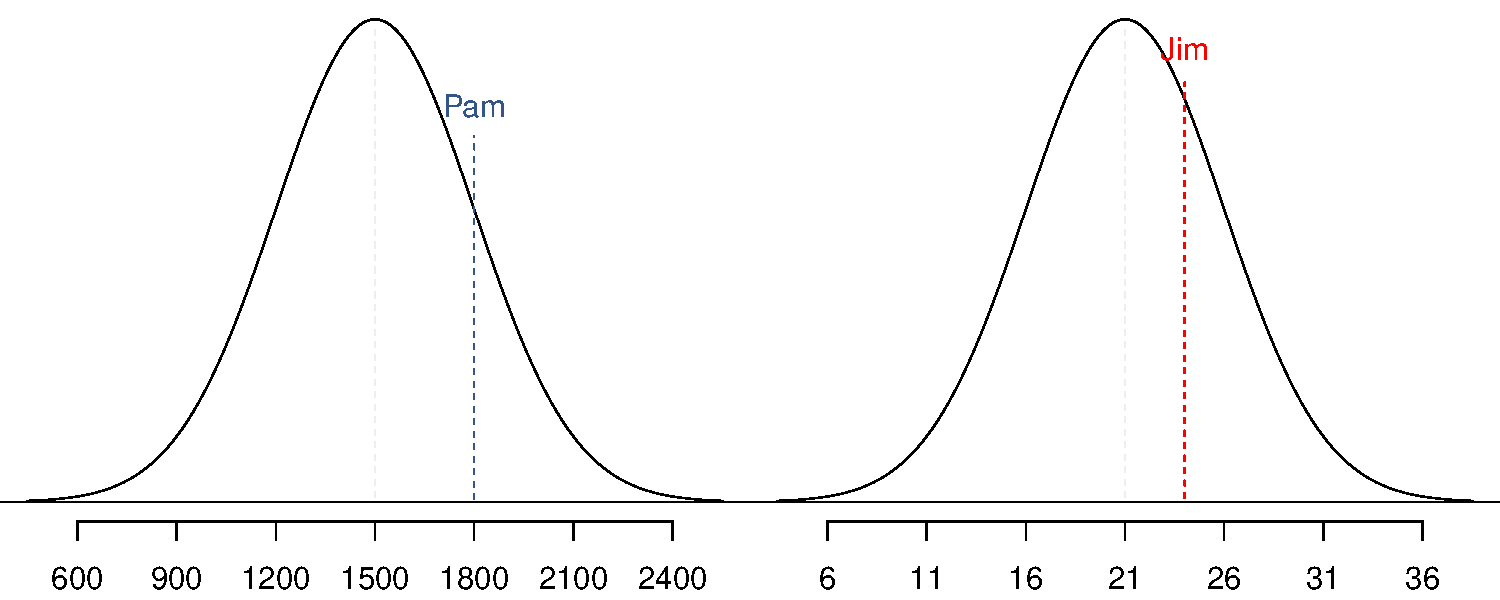
\includegraphics[width=\textwidth]{4-1_normal_distribution/figures/satActNormals/satActNormals}
\end{center}

\end{frame}

%%%%%%%%%%%%%%%%%%%%%%%%%%%%%%%%%%%%

\begin{frame}
\frametitle{Zスコアによる標準化}

これら2つの生の点数を直接比較することはできないため、代わりに各観測値が平均から何標準偏差離れているかを比較する。

\begin{itemize}

\item パムのスコアは平均より $\frac{1800 - 1500}{300} = 1$ 標準偏差上にある。

\item ジムのスコアは平均より $\frac{24 - 21}{5} = 0.6$ 標準偏差上にある。

\end{itemize}

\begin{center}
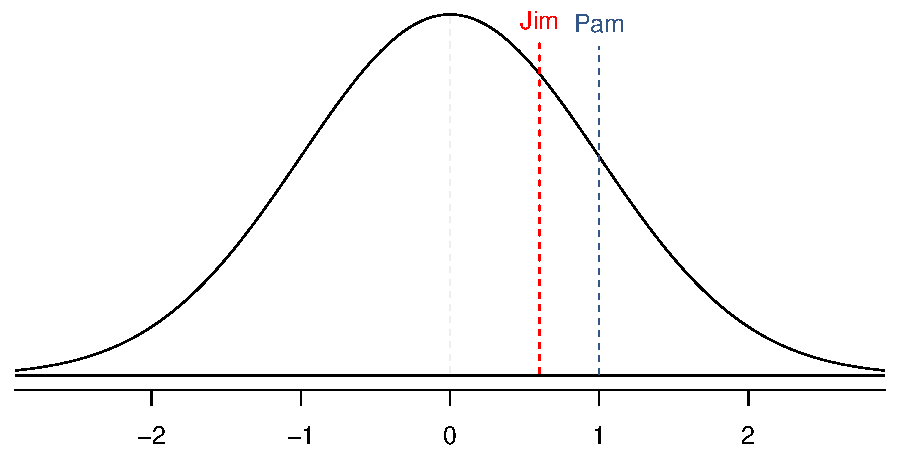
\includegraphics[width=0.7\textwidth]{4-1_normal_distribution/figures/satActNormals/satActNormalsStandardized}
\end{center}

\end{frame}

%%%%%%%%%%%%%%%%%%%%%%%%%%%%%%%%%%%%

\begin{frame}
\frametitle{Zスコアによる標準化（続き）}

\begin{itemize}

\item これらは\hl{標準化スコア}、または\hl{Zスコア}と呼ばれる。

\item 観測値の Zスコアは、それが平均から何標準偏差上または下にあるかを示す。
\formula{\[Z = \frac{\text{観測値} - \text{平均}}{SD}\]}

\item Zスコアはどんな形の分布に対しても定義できるが、分布が正規分布の場合にのみZスコアを使ってパーセンタイルを計算できる。

\item 平均から2SD以上離れている観測値（$|Z| > 2$）は通常、異常値と見なされる。

\end{itemize}

\end{frame}

%%%%%%%%%%%%%%%%%%%%%%%%%%%%%%%%%%%%

\begin{frame}
\frametitle{パーセンタイル}

\begin{itemize}

\item \hl{パーセンタイル}とは、ある特定のデータ点より下に位置する観測値の割合のことである。

\item グラフ的には、パーセンタイルはその観測値の左側の確率分布曲線の下の面積である。

\end{itemize}

\begin{center}
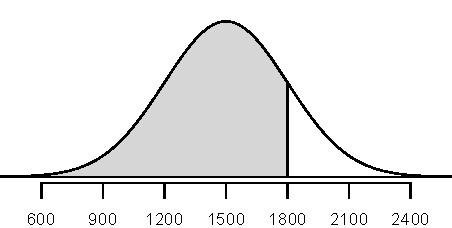
\includegraphics[width=0.7\textwidth]{4-1_normal_distribution/figures/satBelow1800/satBelow1800}
\end{center}

\end{frame}

%%%%%%%%%%%%%%%%%%%%%%%%%%%%%%%%%%%%

\subsection{裾確率の求め方}

%%%%%%%%%%%%%%%%%%%%%%%%%%%%%%%%%%%%

\begin{frame}[fragile]
\frametitle{パーセンタイルの計算 --- 計算機を使う}

曲線の下の面積（パーセンタイル）を計算するには様々な方法がある：

\begin{itemize}
\item R：
\end{itemize}
\begin{beamerboxesrounded}[shadow = false, lower = code body]{}
{\small \begin{verbatim}
> pnorm(1800, mean = 1500, sd = 300)
[1] 0.8413447
\end{verbatim}
}
\end{beamerboxesrounded}
\begin{itemize}
\item アプレット：{\small \webURL{https://gallery.shinyapps.io/dist_calc/}}
\begin{center}
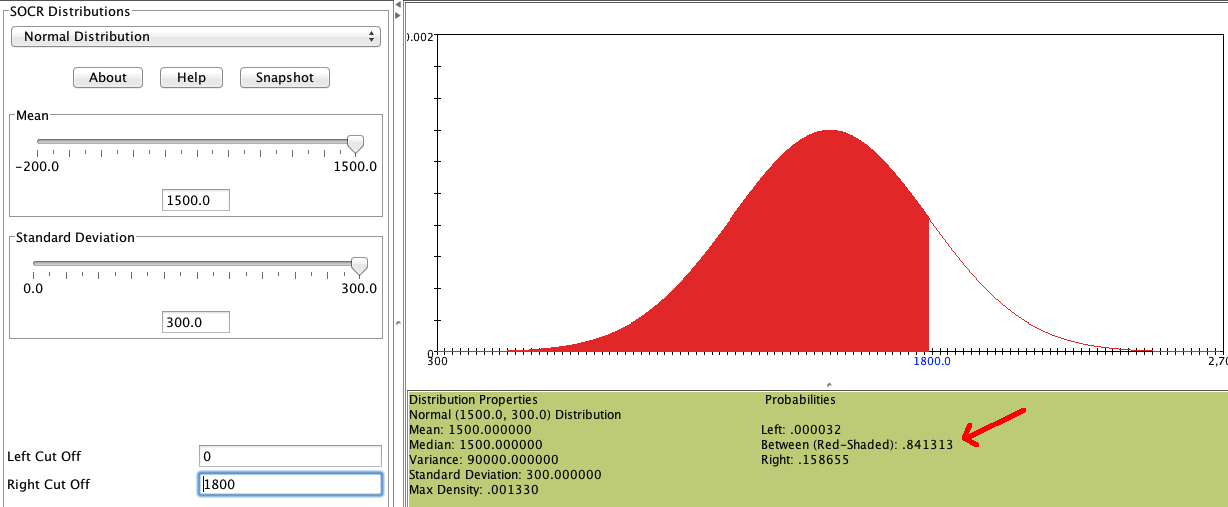
\includegraphics[width=0.8\textwidth]{4-1_normal_distribution/figures/applet}
\end{center}

\end{itemize}


\end{frame}

%%%%%%%%%%%%%%%%%%%%%%%%%%%%%%%%%%%%

\begin{frame}[fragile]
\frametitle{パーセンタイルの計算 --- 表を使う}

{\footnotesize
\begin{tabular}{c | >{\columncolor[gray]{0.6}[0pt]}rrrrr | rrrrr |}
  \cline{2-11}
&&&& \multicolumn{4}{c}{$Z$ の小数第2位} &&& \\
  \cline{2-11}
$Z$ & 0.00 & 0.01 & 0.02 & 0.03 & 0.04 & 0.05 & 0.06 & 0.07 & 0.08 & 0.09 \\
  \hline
  \hline
0.0 & \tiny{0.5000} & \tiny{0.5040} & \tiny{0.5080} & \tiny{0.5120} & \tiny{0.5160} & \tiny{0.5199} & \tiny{0.5239} & \tiny{0.5279} & \tiny{0.5319} & \tiny{0.5359} \\
  0.1 & \tiny{0.5398} & \tiny{0.5438} & \tiny{0.5478} & \tiny{0.5517} & \tiny{0.5557} & \tiny{0.5596} & \tiny{0.5636} & \tiny{0.5675} & \tiny{0.5714} & \tiny{0.5753} \\
  0.2 & \tiny{0.5793} & \tiny{0.5832} & \tiny{0.5871} & \tiny{0.5910} & \tiny{0.5948} & \tiny{0.5987} & \tiny{0.6026} & \tiny{0.6064} & \tiny{0.6103} & \tiny{0.6141} \\
  0.3 & \tiny{0.6179} & \tiny{0.6217} & \tiny{0.6255} & \tiny{0.6293} & \tiny{0.6331} & \tiny{0.6368} & \tiny{0.6406} & \tiny{0.6443} & \tiny{0.6480} & \tiny{0.6517} \\
  0.4 & \tiny{0.6554} & \tiny{0.6591} & \tiny{0.6628} & \tiny{0.6664} & \tiny{0.6700} & \tiny{0.6736} & \tiny{0.6772} & \tiny{0.6808} & \tiny{0.6844} & \tiny{0.6879} \\
  \hline
  0.5 & \tiny{0.6915} & \tiny{0.6950} & \tiny{0.6985} & \tiny{0.7019} & \tiny{0.7054} & \tiny{0.7088} & \tiny{0.7123} & \tiny{0.7157} & \tiny{0.7190} & \tiny{0.7224} \\
  0.6 & \tiny{0.7257} & \tiny{0.7291} & \tiny{0.7324} & \tiny{0.7357} & \tiny{0.7389} & \tiny{0.7422} & \tiny{0.7454} & \tiny{0.7486} & \tiny{0.7517} & \tiny{0.7549} \\
  0.7 & \tiny{0.7580} & \tiny{0.7611} & \tiny{0.7642} & \tiny{0.7673} & \tiny{0.7704} & \tiny{0.7734} & \tiny{0.7764} & \tiny{0.7794} & \tiny{0.7823} & \tiny{0.7852} \\
  0.8 & \tiny{0.7881} & \tiny{0.7910} & \tiny{0.7939} & \tiny{0.7967} & \tiny{0.7995} & \tiny{0.8023} & \tiny{0.8051} & \tiny{0.8078} & \tiny{0.8106} & \tiny{0.8133} \\
  0.9 & \tiny{0.8159} & \tiny{0.8186} & \tiny{0.8212} & \tiny{0.8238} & \tiny{0.8264} & \tiny{0.8289} & \tiny{0.8315} & \tiny{0.8340} & \tiny{0.8365} & \tiny{0.8389} \\
  \hline
  \hline
\rowcolor[gray]{.6}
  1.0 & \orange{\tiny{0.8413}} & \tiny{0.8438} & \tiny{0.8461} & \tiny{0.8485} & \tiny{0.8508} & \tiny{0.8531} & \tiny{0.8554} & \tiny{0.8577} & \tiny{0.8599} & \tiny{0.8621} \\
  1.1 & \tiny{0.8643} & \tiny{0.8665} & \tiny{0.8686} & \tiny{0.8708} & \tiny{0.8729} & \tiny{0.8749} & \tiny{0.8770} & \tiny{0.8790} & \tiny{0.8810} & \tiny{0.8830} \\
  1.2 & \tiny{0.8849} & \tiny{0.8869} & \tiny{0.8888} & \tiny{0.8907} & \tiny{0.8925} & \tiny{0.8944} & \tiny{0.8962} & \tiny{0.8980} & \tiny{0.8997} & \tiny{0.9015} \\
\end{tabular}
}

\end{frame}

%%%%%%%%%%%%%%%%%%%%%%%%%%%%%%%%%%%%

\subsection{正規確率の例}

%%%%%%%%%%%%%%%%%%%%%%%%%%%%%%%%%%%%

\begin{frame}
\frametitle{シックスシグマ}

「\textit{シックスシグマプロセス}という言葉は、グラフに示すように、プロセス平均と最も近い規格限界との間に6つの標準偏差がある場合、事実上すべての製品が規格を満たすという考え方に由来する。」

\begin{center}
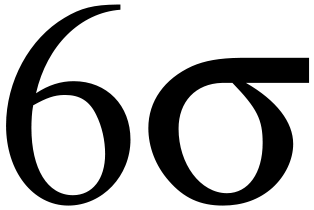
\includegraphics[width=0.35\textwidth]{4-1_normal_distribution/figures/sixsigma}
\end{center}

\ct{\webURL{http://en.wikipedia.org/wiki/Six_Sigma}}

\end{frame}

%%%%%%%%%%%%%%%%%%%%%%%%%%%%%%%%%%%%

\begin{frame}
\frametitle{品質管理}

\dq{{\small ハインツのケチャップ工場では、ケチャップのボトルに入る量が平均36オンス、標準偏差0.11オンスの正規分布に従うとされている。30分ごとに生産ラインからボトルが1本選ばれ、その内容量が正確に記録される。ケチャップの量が35.8オンス未満または36.2オンス超の場合、そのボトルは品質管理検査に不合格となる。ケチャップが35.8オンス未満のボトルは何パーセントか？}}

\soln{
$X$ = ボトル内のケチャップの量とする：$X \sim N(\mu = 36, \sigma = 0.11)$ \\
\twocol{0.4}{0.6}{
\begin{center}
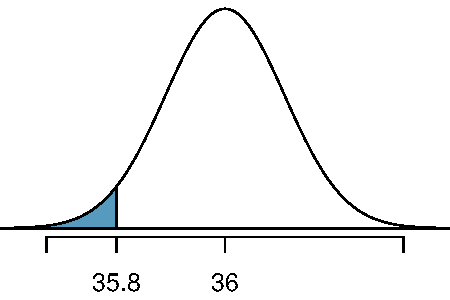
\includegraphics[width=\textwidth]{4-1_normal_distribution/figures/ketchup/ketchupLT358}
\end{center}
}
{
\[ Z = \frac{35.8 - 36}{0.11} = -1.82 \]
}
}

\end{frame}

%%%%%%%%%%%%%%%%%%%%%%%%%%%%%%%%%%%%

\begin{frame}[fragile]
\frametitle{正確な確率の求め方 --- R を使う}

\begin{beamerboxesrounded}[shadow = true, lower = code body]{}
{\small \begin{verbatim}
> pnorm(-1.82, mean = 0, sd = 1)
[1] 0.0344
\end{verbatim}
}
\end{beamerboxesrounded}

$\:$ \\

または

$\:$ \\

\begin{beamerboxesrounded}[shadow = true, lower = code body]{}
{\small \begin{verbatim}
> pnorm(35.8, mean = 36, sd = 0.11)
[1] 0.0345
\end{verbatim}
}
\end{beamerboxesrounded}


\end{frame}

%%%%%%%%%%%%%%%%%%%%%%%%%%%%%%%%%%%%%

\begin{frame}[shrink=15]
\frametitle{練習問題}

\pq{品質管理検査に\underline{合格}するボトルは何パーセントか？}

\vspace{-0.5cm}
\begin{multicols}{2}
\begin{enumerate}[(a)]
\item 1.82\%
\item 3.44\%
\item 6.88\%
\solnMult{93.12\%}
\item 96.56\%
\item[]
\end{enumerate}
\end{multicols}

\soln{
\vspace{-0.5cm}
\begin{columns}[c]
\column{0.3\textwidth}
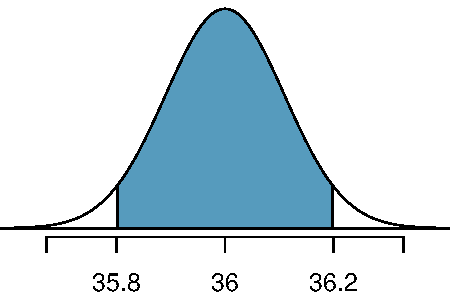
\includegraphics[width=\textwidth]{4-1_normal_distribution/figures/ketchup/ketchupBET}
\column{0.05\textwidth}
=
\column{0.3\textwidth}
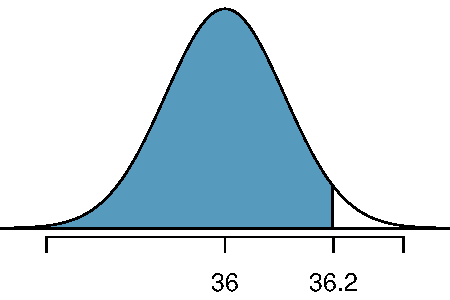
\includegraphics[width=\textwidth]{4-1_normal_distribution/figures/ketchup/ketchupLT362}
\column{0.05\textwidth}
-
\column{0.3\textwidth}
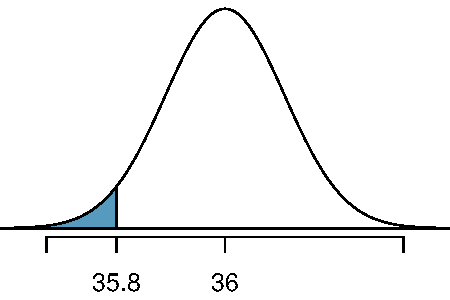
\includegraphics[width=\textwidth]{4-1_normal_distribution/figures/ketchup/ketchupLT358}
\end{columns}
\begin{eqnarray*}
Z_{35.8} &=& \frac{35.8 - 36}{0.11} = -1.82 \\
Z_{36.2} &=& \frac{36.2 - 36}{0.11} = 1.82 \\
P(35.8 < X < 36.2) &=& P(-1.82 < Z < 1.82) = 0.9656 - 0.0344 = 0.9312
\end{eqnarray*}
}

\end{frame}

%%%%%%%%%%%%%%%%%%%%%%%%%%%%%%%%%%%%

\begin{frame}[fragile]
\frametitle{カットオフ点の求め方}

\dq{健康な人間の体温は平均98.2$\degree$F、標準偏差0.73$\degree$Fの正規分布にほぼ従う。人間の体温の下位3\%のカットオフは何$\degree$Fか？}

\twocol{0.3}{0.7}
{
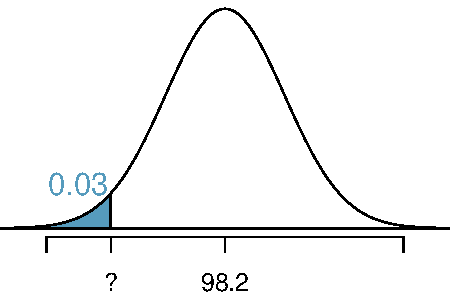
\includegraphics[width=\textwidth]{4-1_normal_distribution/figures/temp/tempLOW3PERC}
}
{
{\small
\begin{eqnarray*}
P(X < x) &=& 0.03 \\
  &\rightarrow& P(Z < \orange{-1.88}) = 0.03 \\
Z &=& \frac{\text{観測値}~-~\text{平均}}{SD} \\
  &\rightarrow& \frac{x - 98.2}{0.73} = -1.88 \\
x &=& (-1.88 \times 0.73) + 98.2 = 96.8\degree F
\end{eqnarray*}
}
}
$\:$ \\
\begin{beamerboxesrounded}[shadow = true, lower = code body]{}
{\small \begin{verbatim}
> qnorm(0.03)
[1] -1.880794
\end{verbatim}
}
\end{beamerboxesrounded}

\ct{Mackowiak, Wasserman, and Levine (1992), \textit{A Critical Appraisal of 98.6 Degrees F, the Upper Limit of the Normal Body Temperature, and Other Legacies of Carl Reinhold August Wunderlick}.}

\end{frame}

%%%%%%%%%%%%%%%%%%%%%%%%%%%%%%%%%%%

\begin{frame}[fragile,shrink=10]
\frametitle{練習問題}

\pq{健康な人間の体温は平均98.2$\degree$F、標準偏差0.73$\degree$Fの正規分布にほぼ従う。人間の体温の上位10\%のカットオフは何$\degree$Fか？}

\vspace{-0.5cm}
\begin{multicols}{2}
\begin{enumerate}[(a)]
\item 97.3$\degree$F
\solnMult{99.1$\degree$F}
\item 99.4$\degree$F
\item 99.6$\degree$F
\end{enumerate}
\end{multicols}

\soln{
\vspace{-0.5cm}
\twocol{0.3}{0.7}
{
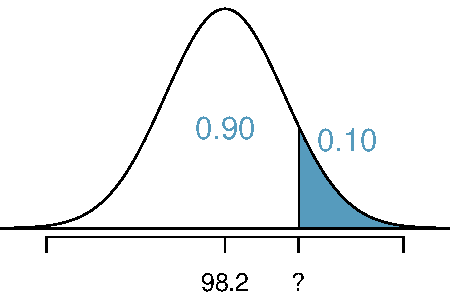
\includegraphics[width=\textwidth]{4-1_normal_distribution/figures/temp/tempHIGH10PERC}
}
{
\begin{eqnarray*}
P(X > x) &=& 0.10 \rightarrow P(Z < \orange{1.28}) = 0.90 \\
Z &=& \frac{\text{観測値}~-~\text{平均}}{SD} \rightarrow \frac{x - 98.2}{0.73} = 1.28 \\
x &=& (1.28 \times 0.73) + 98.2 = 99.1
\end{eqnarray*}
}
}

\end{frame}

%%%%%%%%%%%%%%%%%%%%%%%%%%%%%%%%%%%

\subsection{68-95-99.7則}

%%%%%%%%%%%%%%%%%%%%%%%%%%%%%%%%%%%%

\begin{frame}
\frametitle{68-95-99.7則}

\begin{itemize}

\item ほぼ正規分布に従うデータでは、
\begin{itemize}
\item 約68\%が平均から1SD以内に収まる、
\item 約95\%が平均から2SD以内に収まる、
\item 約99.7\%が平均から3SD以内に収まる。
\end{itemize}

\item 平均から4SD、5SD、またはそれ以上離れた観測値が存在することもあるが、データがほぼ正規分布に従う場合、このような出来事は非常にまれである。

\end{itemize}

\begin{center}
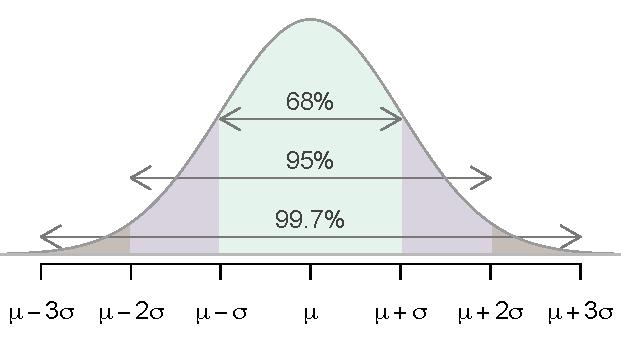
\includegraphics[width=0.7\textwidth]{4-1_normal_distribution/figures/6895997/6895997}
\end{center}

\end{frame}

%%%%%%%%%%%%%%%%%%%%%%%%%%%%%%%%%%%%

\begin{frame}
\frametitle{68-95-99.7則を使った変動性の記述}

SAT のスコアは平均1500、標準偏差300の正規分布にほぼ従う。

\begin{itemize}

\item SAT で1200〜1800点の間に収まる学生は約68\%。

\item SAT で900〜2100点の間に収まる学生は約95\%。

\item SAT で600〜2400点の間に収まる学生は約99.7\%。

\end{itemize}

\begin{center}
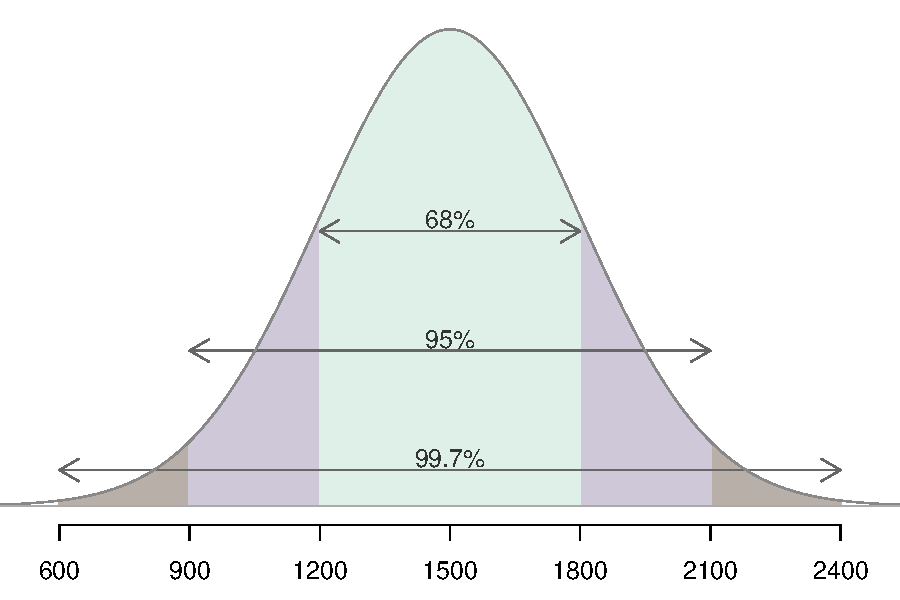
\includegraphics[width=0.65\textwidth]{4-1_normal_distribution/figures/sat_empirical/sat_empirical}
\end{center}

\end{frame}

%%%%%%%%%%%%%%%%%%%%%%%%%%%%%%%%%%%%

\begin{frame}[fragile]
\frametitle{平日の睡眠時間}

\begin{center}
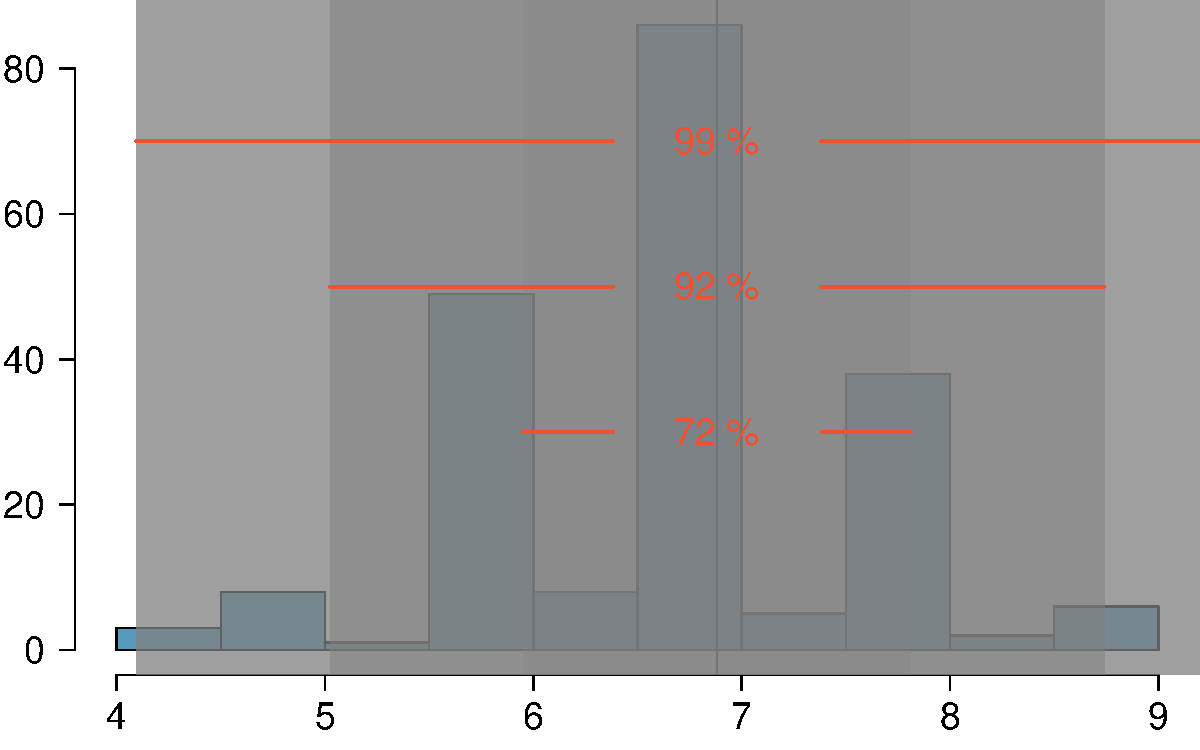
\includegraphics[width=0.75\textwidth]{4-1_normal_distribution/figures/sleep/sleep-hist-sd3}
\end{center}
\vspace{-0.25cm}
\begin{itemize}
\item 平均 = 6.88 時間、SD = 0.92 時間
\item データの72\%は平均から1SD以内：$6.88 \pm 0.93$
\item データの92\%は平均から2SD以内：$6.88 \pm 2 \times 0.93$
\item データの99\%は平均から3SD以内：$6.88 \pm 3 \times 0.93$
\end{itemize}

\end{frame}

%%%%%%%%%%%%%%%%%%%%%%%%%%%%%%%%%%%%

\begin{frame}
\frametitle{練習問題}

\pq{次のうち\underline{誤り}はどれか？}

\begin{enumerate}[(a)]
\item 右に歪んだ分布では、Zスコアの大半は負である。
\solnMult{歪んだ分布では、平均のZスコアが0と異なる場合がある。}
\item 正規分布では、IQR は $2 \times SD$ より小さい。
\item Zスコアは、あるデータ点が分布の残りのデータと比べてどれだけ異常かを判断するのに役立つ。
\end{enumerate}

\end{frame}

%%%%%%%%%%%%%%%%%%%%%%%%%%%%%%%%%%%%
